\subsection{QuizziPedia::Back-End::App::Controllers::Errors}
\subsubsection{Informazioni generali}
\label{QuizziPedia::Back-End::App::Controllers::Errors}
\begin{figure}[ht]
	\centering
	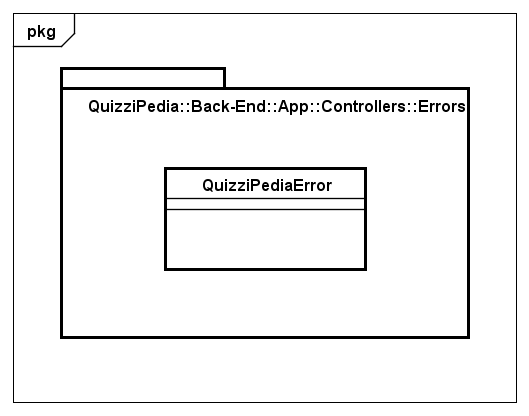
\includegraphics[scale=0.45]{UML/Package/QuizziPedia_Back-End_App_Controllers_Errors.png}
	\caption{QuizziPedia::Back-End::App::Controllers::Errors}
\end{figure}
\FloatBarrier


	\begin{itemize}
		\item \textbf{Descrizione}:
		\textit{package\ped{G}} contenente i controllers per la gestione degli errori specifici.
		\item \textbf{Padre}: \texttt{Controllers}
	\end{itemize}
\subsubsection{Classi}
\paragraph{QuizziPedia::Back-End::App::Controllers::Errors::QuizziPediaError}
\begin{figure}[ht]
	\centering
	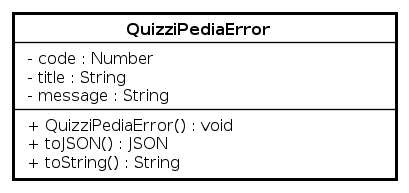
\includegraphics[scale=0.45]{UML/Classi/Back-End/QuizziPedia_Back-End_App_Controllers_Errors_QuizziPediaError.png}
	\caption{QuizziPedia::Back-End::App::Controllers::QuizziPediaError}
\end{figure}
\FloatBarrier


	\begin{itemize}
		\item \textbf{Descrizione}:
		classe che contiene gli errori. Esegue la costruzione del messaggio d'errore specifico per i moduli di \texttt{QuizziPedia::Back-End::App}.
		\item \textbf{Utilizzo}:
		viene utilizzato da \texttt{ErrorsHandler} quando di verifica un errore specifico relativo alle classi di \texttt{QuizziPedia::Back-End::App}
		\item \textbf{Relazioni con altre classi}:
			 \begin{itemize}
			 	\item \textit{IN} \texttt{ErrorsHandler} \\
			 	Classe middleware\ped{G} per la gestione degli errori. Ritorna al client un oggetto di tipo \texttt{Response} con stato \textit{HTTP\ped{G}} 500 e descrizione dell'errore in formato \textit{JSON\ped{G}}. E' un componente \textit{ConcreteHandler\ped{G}} del \textit{design pattern\ped{G}} \textit{Chain of responsability\ped{G}}.
			 \end{itemize}
		\item \textbf{Attributi}:
			 \begin{itemize}
			 	\item \texttt{- code : Number}\\
			 	Campo dati contenente il codice dell'errore;
			 	\item \texttt{- message : String}\\
			 	Campo dati contenente il messaggio che corrisponde all'errore;
			 	\item \texttt{- title : String}\\
			 	Campo dati contenente il titolo dell'errore in forma di stringa.
			 \end{itemize}
		\item \textbf{Metodi}:
			\begin{itemize}
				\item \texttt{+ QuizziPediaError(err: Number)}\\
				Costruttore della classe QuizziPediaError.\\
				\textbf{Parametri}:
				\begin{itemize}
					\item \texttt{err: Number}\\
					Rappresenta il codice identificativo dell'errore.
				\end{itemize}
				\item \texttt{+ toJSON()}\\
				Metodo che ritorna l'errore in formato JSON;
				\item \texttt{+ toString()}\\
				Metodo che effettua una concatenazione dei campi dati dell'errore e li ritorna in formato String.
			\end{itemize}
	\end{itemize}